\label{fundamentacao_teorica}

%%%%%%%%%%%%%%%%%%%%%%%%%%%%%%%%%%%%%%%%%%%%%%%%%%%%%%%%%%%%%%%%%%%%%%%%%%%%%%%

\newcommand{\texCommand}[1]{\texttt{\textbackslash{#1}}}%

\newcommand{\exemplo}[1]{%
\vspace{\baselineskip}%
\noindent\fbox{\begin{minipage}{\textwidth}#1\end{minipage}}%
\\\vspace{\baselineskip}}%

\newcommand{\exemploVerbatim}[1]{%
\vspace{\baselineskip}%
\noindent\fbox{\begin{minipage}{\textwidth}%
#1\end{minipage}}%
\\\vspace{\baselineskip}}%

%%%%%%%%%%%%%%%%%%%%%%%%%%%%%%%%%%%%%%%%%%%%%%%%%%%%%%%%%%%%%%%%%%%%%%%%%%%%%%%

Este capítulo descreve a revisão conceitual sobre as tecnologias relacionadas ao tema deste projeto. 

%%%%%%%%%%%%%%%%%%%%%%%%%%%%%%%%%%%%%%%%%%%%%%%%%%%%%%%%%%%%%%%%%%%%%%%%%%%%%%%%

\section{Monitoramento de sistemas distribuídos}%

O monitoramento é forma utilizada para acompanhar ou observar o andamento de um fluxo ou processo, na área de tecnologia da informação é responsável por verificar e coletar informações sobre funcionamento de ativos de rede ou serviços, com propósito de apresentar informações mais resumidas e favoráveis em painéis ou sistemas para a realização de monitoramento\cite{de2014indicadores}. O monitoramento é necessário para uma série de fins, incluindo a verificação de status, solução de problemas, ajustes de desempenho e depuração\cite{hollingsworth2003instrumentation}. 

A intenção de monitorar ativos de rede e serviços, é mante-los sempre disponíveis, seja pelo mau funcionamento de um ativo de rede, serviço ou por uma indisponibilidade(queda de energia ou internet). Como mencionado anteriormente o ato de acompanhar o funcionamento desses recursos propõem ao gestores desse processos encontrar uma forma mais visível e gerenciável para solucionar problemas, alertar sobre possíveis falhas ou até determinar uma situação para o retorno automático desses serviços. 

O CPD, atualmente possui um serviço que executa o monitoramento em tempo de execução, porém a forma utilizada para o monitoramento foi a leitura do arquivo de \textit{log}, pois havia um grande preocupação com \textit{trade-off} gerado. A fim de obter melhor custo de monitoramento x desempenho tomou-se a decisão pela coleta das informações de monitoramento por meio dos \textit{logs} gerados pelo ErlangMS \cite{filgueirasmonitoramento}.    

O monitoramento implantado no \acrshort{CPD} para acompanhamento dos sistemas e serviços(\textit{web services}), desenvolvidos pela unidade de desenvolvimento \textit{software} utilizando o Barramentos de serviços ErlangMS, não possui um acompanhamento especifico no funcionamento dos seus serviços, visto que há casos e relatos de usuários que acessam os sistemas, realizam a autenticação, clicam nos menus, mas nada aparece como resultado das pesquisas e funcionalidades dos sistemas. Por dispor de uma arquitetura orientada a serviços a camada de apresentação funciona normalmente, mas os recursos(\textit{web services}) encontram-se indisponíveis.

Sistemas distribuídos podem ser interpretados como aplicações distintas que possuem um \textit{middleware} que realize algum tipo de conexão entre as aplicações \cite{penteado2012jmonitor}. Esses sistemas ou aplicações podem funcionar com seus serviços de forma independente, ou dependente de outros serviços de aplicações distintas, o funcionamento desses serviços são essenciais, principalmente os que são dependentes, por esse motivo a implantação do monitoramento de sistemas distribuídos é utilizada para um melhor acompanhamento e gerenciamento das aplicações e serviços para verificar o funcionamento e disponibilidade.   

%%%%%%%%%%%%%%%%%%%%%%%%%%%%%%%%%%%%%%%%%%%%%%%%%%%%%%%%%%%%%%%%%%%%%%%%%%%%%%%%

\section{Arquitetura Orientada a Serviços - SOA}

A Arquitetura Orientada a Serviços pode ser descrita com um estilo arquitetural capaz de realizar a comunicação entre aplicações heterogêneas por meio de mensagens\cite{fraser2007service}. É comum que essas aplicações possuam estruturas e linguagens completamente distintas, pois as aplicações envolvidas, normalmente independem umas das outras e precisam que essa comunicação aconteça, mas para que haja a comunicação interoperável entre as aplicações é previsto na arquitetura \acrshort{SOA} que a as funcionalidade possam ser disponibilizadas por meio de serviços(\textit{web services}) em componentes distribuídos, que ao mesmo tempo que possam fornece-los possam também consumi-los\cite{sward2011service,bianco2011architecting}.

Com o aumento da utilização da arquitetura percebeu-se a necessidade de discuções e definições afim abraçar os conceitos da arquitetura \acrshort{SOA}, com as discuções decidu-se não apenas criar conceitos, mas tabém orientações  afim  de guiar as organizações de maneira consistente e sustentável, de modo a agregar valor ao negócio, com maior agilidade e efetividade de custos, em alinhamento com a dinâmica das necessidades de negócio, e foi a apartir desse movimento que sugiu o Manifesto \acrshort{SOA} \cite{erl2009soa} priorizando os seguintes itens:

\begin{itemize}

\item Valor do negócio em relação a estratégia técnica;

\item Objetivos estratégicos em relação a benefícios específicos de projetos;

\item Interoperabilidade intrínseca em relação a integração personalizada;

\item Serviços compartilhados em relação a implementações de propósito específico;

\item Flexibilidade em relação a otimização; e

\item Refinamento evolutivo em relação a busca da perfeição inicial.

\end{itemize}

Para realização da comunicação entre as aplicações ou serviços em componentes distribuídos no estilo arquitetural \acrshort{SOA}, \cite{clements2002documenting} descreve em seu trabalho que a comunicação poderá ser executada por meio de um itermediador ou na falta dele poderá ser realizada ponto-a-ponto, entre os intermediadores o estilo arquitetural \acrshort{SOA} dispõe dos seguintes tipos de componentes que compõem uma arquitetura orientada a serviços, são eles \cite{bass2003software}:

\begin{itemize}

\item Prestador de serviços;

\item Consumidores de serviço;

\item \acrfull{ESB};

\item Registro de serviços;

\item Server Orchestration; 

\item \acrfull{SOAP}.

\item \acrfull{REST}

\item Conector de mensagens assíncronas

\end{itemize}

Com a utilização desses componentes \cite{bass2003software} trata como principal benefício de uma arquitetura \acrshort{SOA} a interoperabilidade, pois permite que aplicações, dispositivos, sistemas e serviços hetorogeneos possam realizar a comunicação entre si, fornecendo e consumindo informações  de forma itegrada. 

O \acrshort{CPD} para implementação e implantação da arquitetura \acrshort{SOA} na modernização dos seus sistemas, escolheu como componente o \acrshort{ESB} e como plataforma o barramento ErlangMS\cite{Agilar},que atua como intermediador prestando serviço de mensageria.

%%%%%%%%%%%%%%%%%%%%%%%%%%%%%%%%%%%%%%%%%%%%%%%%%%%%%%%%%%%%%%%%%%%%%%%%%%%%%%%%

\section{ESB}

Um componente \acrshort{ESB} é responsável por fornecer serviço de infraestrutura e mediar a comunicação por meio de serviços entre aplicações consumidoras e fornecedoras de serviços, fazendo de forma uniforme a transmissão das mensagens por meio de um protocolo ou tecnologia, utilizando conectores do tipo \textit{Call-return}, onde os mais comuns e também mais utilizados no mercado são o \acrshort{SOAP} e o \acrshort{REST}  	 \cite{clements2002documenting}.

Para a implementação de um \acrshort{ESB} no estilo \acrshort{SOA} devem ser seguidos alguns itens primordiais para o funcionamento, mas primeiro a organização ou instituição deverá avaliar as tecnologias utilizadas em seus sistemas ou serviços, visto que, a complexidade de uma arquitetura \acrshort{SOA} é alta, e dependendo da situação não é necessário a implementação ou implantação de um \acrshort{ESB} quando por exemplo, uma organização que  possui em sua arquitetura de sistemas a mesma linguagem, plataforma e tecnologia, podendo fazer a comunicação ou troca de mensagens ponto-a-ponto\cite{bianco2011architecting}. No caso em que existe a necessidade da implementação ou implantação de um \acrshort{ESB}, a padronização e táticas descritas em \cite{bianco2011architecting} que devem ser seguidas, e de acordo com \cite{erl2009soa} possuem as seguintes características, são elas:

\begin{itemize}

\item Roteamento Intermediário: Um serviço de roteamento genérico intercepta mensagens e com base no encaminhamento a lógica que determina para onde as mensagens devem ser enviadas.

\begin{itemize}

\item Balanceamento de carga: Possuir um \textit{Failover} para um \textit{backup} no caso de o serviço de destino 	primário não estar disponível.

\item{Seleção da versão do Serviço: Verificar se os pedidos são enviados para versões compatíveis de um serviço para     suportar compatibilidade com versões anteriores durante os períodos de transição}.

\item Serviço de seleção com base em dados da mensagem: Verificar se pedidos de clientes são enviados para um componente de processamento mais rápido.

\item Regras de controle de acesso: Analisar um pedido de um usuário não autenticado é encaminhado para um início de sessão página.

\item Tratamento de exceções: Apresentar uma mensagem de erro de resposta que é redirecionada para um serviço responsável para manipulação de exceção centralizada.

\end{itemize}

\item O \textit{Service Broker}: Integrar componentes que foram desenvolvidos em diferentes linguagem por diferentes organizações.

\begin{itemize}

\item Modelo de Transformação de Dados: Os dados enviados do consumidor de serviços numa dada estrutura transforma-se em uma estrutura diferente, que está prevista para o prestador de serviços.

\item Conversão de Formato de dados: Usar sempre consumidor de serviço e o fornecedor precisa de trocar dados representados em diferentes formatos como por exemplo, \acrshort{XML}, \acrshort{CSV}, \acrshort{JSON}.

\item Protocolo \textit{Bridging}: O consumidor de serviço envia uma solicitação usando um protocolo e o \textit{Service Broker} intercepta o pedido e o converte para um pedido ao fornecedor do serviço usando um protocolo diferente.

\end{itemize}

\item Mensagens \textit{Asynchronous}: Alguns \acrshort{ESB}s fornecem capacidade suficiente para que o sistema de mensagens permita que os pedidos e respostas de um serviço possam ser trocados através de canais de mensagens.

\item Interceptor: Alguns \acrshort{ESB}s oferecem a capacidade de configurar interceptores, que são elementos de software que são ativados para todas as solicitações e respostas.

\end{itemize}

O \acrshort{ESB} a ser implementado deve possuir vantagens e benefícios que uma arquitetura \acrshort{SOA} pode fornecer, para alcança-los \cite{bianco2011architecting} cita os seguintes itens(Atributos de Qualidade), como representação de um \acrshort{ESB} padronizado e operável, o atendimento à esses itens são de suma importância, são eles:

\begin{itemize}

\item Interoperabilidade: O \acrshort{ESB} permite que sistemas diferentes possam interoperar, por meio de protocolos de comunicação e tecnologias de implementação. 

\item Modificabilidade: A capacidade de executar a transformação do modelo de dados que permite a implantação de novas versões de um serviço sem interromper consumidores de serviços existentes. 

\item Confiabilidade: Quando o receptor de uma solicitação de serviço ou resposta falhou, e o ESB cria ou gera uma fila para que mensagem seja executa quando o serviço estiver disponível novamente. 

\item Segurança: O \acrshort{ESB} pode incluir a funcionalidade de controle de acesso. Pode aplicar a autenticação e regras de autorização em trocas de mensagens de serviço.

\end{itemize}

Como desafio o \acrshort{ESB} deve responder a altura seus \textit{trade-offs},  principalmente em uma arquitetura complexa como essa, entre os desafios que deverão ser suportados, para um bom funcionamento da plataforma, \cite{bianco2011architecting} cita a:

\begin{itemize}

\item Manutenibilidade: Ter cuidado e atenção ao especificar demais a codificação do ESB, ao ponto de restringir comunicação com outras tecnologias. 
 	
\item Performance: Não permitir a perda comprometedora no desempenho do \acrshort{ESB} por conta das logicas de roteamento ou interpretação dos dados durante a comunicação.

\item Segurança: verificar a configuração a fim de evitar acessos não autorizados ao \acrshort{ESB}.

\item Disponibilidade: O \acrshort{ESB} pode ser um ponto único de falha no sistema.

\end{itemize}

%%%%%%%%%%%%%%%%%%%%%%%%%%%%%%%%%%%%%%%%%%%%%%%%%%%%%%%%%%%%%%%%%%%%%%%%%%%%%%%%

\section{REST}

A Transferência de Estado Representacional - \acrshort{REST} pode ser definida como um estilo arquitetural hibrido derivado de vários dos estilos arquiteturais baseados em rede e que define um conjunto de restrições e propriedades baseados no protocolo de comunicação \acrshort{HTTP}, com a intenção de fornecer a interoperabilidade entre sistemas, serviços e aplicações distribuídas conectadas a rede mundial de computadores - \acrshort{WWW} para a realização de troca de informações \cite{fielding2000architectural}. Os \textit{web services} compatíveis com \acrshort{REST} permitem que os sistemas solicitantes acessem e manipulem representações textuais de recursos da \textit{Web} utilizando um conjunto uniforme e predefinido de operações sem estado. O estilo arquitetural proposto por Roy Fielding que inspirou a criação do documento de arquitetura definido pelo \acrshort{TAG} - \acrshort{W3C},  quanto muitos outros arquitetos de \textit{softaware}, que o veem como um modelo norteador para construir e padronizar serviços da Web \cite{booth2013web}. O \acrshort{REST} fornece semântica para uniformizar sua interface, principalmente no que tange a  operações para criar, recuperar, atualizar e excluir dados, e  também a possibilidade da utilização de padrões de tecnologia como \acrshort{XML} e o \acrshort{JSON}. 

Em \acrshort{REST} as principais operações por meio do protocolo \acrshort{HTTP} são:

\begin{itemize}

\item POST: Cria uma nova entidade ou recurso. 

\item GET: Recupera a informação de um recurso.

\item PUT: Atualiza os dados de um recurso informado.

\item DELETE: Exclui os dados de um recurso informado.

\end{itemize}

%%%%%%%%%%%%%%%%%%%%%%%%%%%%%%%%%%%%%%%%%%%%%%%%%%%%%%%%%%%%%%%%%%%%%%%%%%%%%%%%

\section{JSON}

\acrfull{JSON} é um formato baseado em texto, de fácil leitura e intepretação para humanos, para a leitura de máquinas o \acrshort{JSON} é baseado em um subconjunto da linguagem de programação \textit{JavaScript}, e por possuir um um padrão, seu funcionamento independe de uma tecnologia ou linguagem de programação, focando principalmento na troca de dados e mensagens \cite{bray2017javascript}.

Por decisão técnica especificamente relacionada a interoperabilidade e o baixo acoplamento o barramento utilizado pelo \acrshort{CPD} o Erlangms, utiliza o \acrshort{JSON} por conta do  baixo\textit{overhead} gerado na troca de mensagens em relação as trocas de mensagens feitas com a utilização protocolo \acrshort{SOAP} com a linguagem \acrshort{WSDL}, e apontando também o nível baixa da curva de aprendizagem para a utilização do \acrshort{JSON}.

%%%%%%%%%%%%%%%%%%%%%%%%%%%%%%%%%%%%%%%%%%%%%%%%%%%%%%%%%%%%%%%%%%%%%%%%%%%%%%%%

\section{ErlangMs}
O Barramento de serviços da \acrshort{UnB} denominado Erlangms foi conceituado em uma disciplina do \acrshort{MPCA} e proposto como trabalho para solucionar alguns problemas relacionados a quantidade de sistemas heterogêneos, defasagem tecnológica das aplicaões e a falta de um padrão de comunicação entre eles no \acrshort{CPD} \cite{Agilar}. 

O Erlangms dispoem de uma arquitetura \acrshort{SOA} utilizando o estilo arquitetural \acrshort{REST} e sua implementação foi feita na liguagem funcional Erlang. O barramento atualmente está implantado no \acrshort{CPD} e  funcionando com um serviço de mensageria. A realização da comunicação e troca de mensagems dos sistemas e clientes é feita por meio de serviços(\textit{web services}) utilizando o formato \acrshort{JSON}. O Erlangms tem sua arquitetura é apresentada na figura \ref{fun:fig:erlangms}

\begin{figure}[h!]
	\begin{center}
	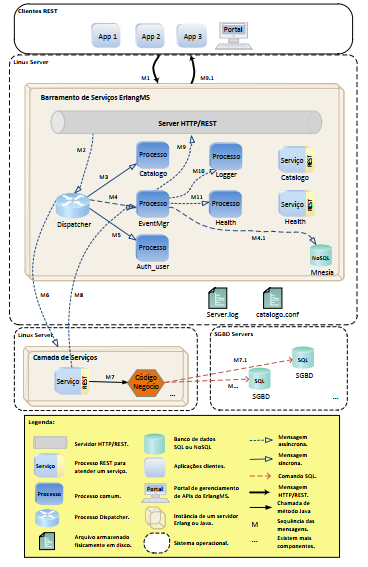
\includegraphics[scale = 1.20]{img/Arquitetura_ErlangMS.png}
		\caption{Arquitetura do trabalho Erlangms descrita por\cite{Agilar}}
		\label{fun:fig:erlangms}
	\end{center}
\end{figure}
%%%%%%%%%%%%%%%%%%%%%%%%%%%%%%%%%%%%%%%%%%%%%%%%%%%%%%%%%%%%%%%%%%%%%%%%%%%%%%%%

\section{Ferramentas de Monitoramento}

\begin{enumerate}
\item Nagios

O Nagios é uma ferramenta de monitoramento de rede baseada na web idealizada e desenvolvida por Ethan Galstad \cite{bin2011new}. O Nagios é projetado para a realizar o acompanhamento de ativos de rede, sistemas e serviços com a finalidade de notificar os usuários e responsáveis pelos ativos de rede, sistema e serviços que estão registrados na ferramenta como contatos emergências, em caso aconteça alguma anomalia ou problema durante o funcionamento da rede, sistemas e serviços.

O Nagios é tratado como uma ferramenta que possui um alta complexidade em sua configuração, pois possui uma gama de recursos e funcionalidades disponíveis para a utilização, devido a grande quantidade de recurcos o Nagios é bastante utilizado ele também possui um grande número de \textit{plug-ins} disponíveis na para a realização do monitoramento podendo personalizar o monitoramnto de serviços como SMTP, POP3, HTTP, PING \cite{lcc2012nagios}. Nesse projeto o Nagios será utlizado com ferramenta de monitoramento dos sistemas e serviços fornecidos pela \acrshort{UnB} com utilização de serviço SMTP para o monitoramento, visto que, o \acrshort{CPD} já utiliza a ferramenta para o monitoramento dos ativos de rede de toda a universidade. 

\begin{figure}[h!]
	\begin{center}
	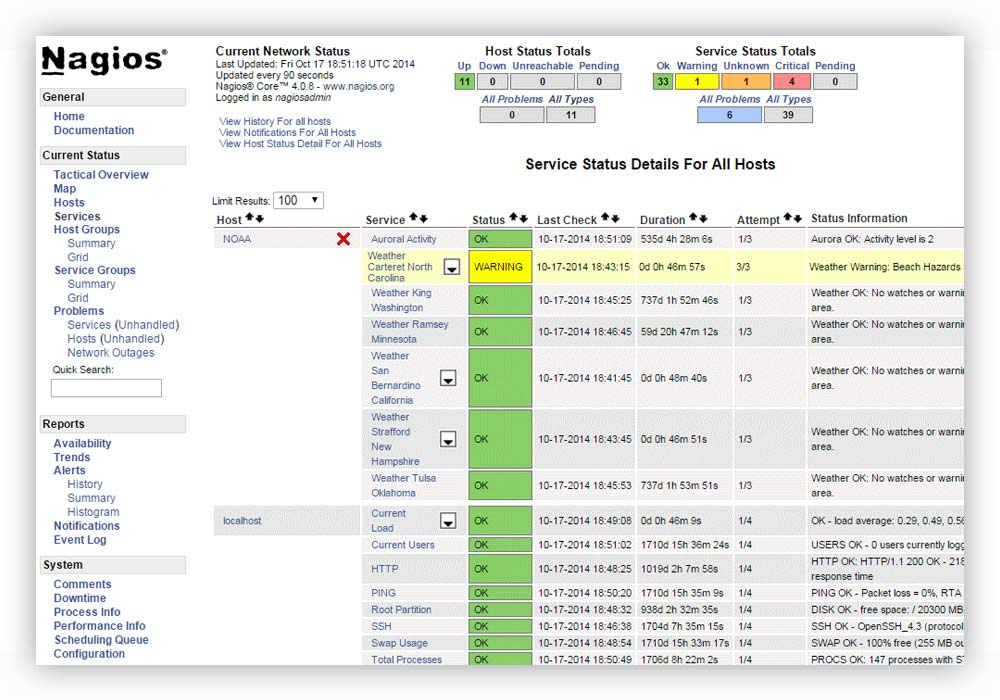
\includegraphics[scale = 0.40]{img/Comprehensive_Monitoring_Drop2.jpg}
		\caption{Monitoramento de componentes\cite{lcc2012nagios}}
		\label{fun:fig:nagios}
	\end{center}
\end{figure}

\item Ganglia
\item Cacti
\item Zabbix
\end{enumerate}

....

%%%%%%%%%%%%%%%%%%%%%%%%%%%%%%%%%%%%%%%%%%%%%%%%%%%%%%%%%%%%%%%%%%%%%%%%%%%%%%%%

\section{Agentes de monitoramento}

....

%%%%%%%%%%%%%%%%%%%%%%%%%%%%%%%%%%%%%%%%%%%%%%%%%%%%%%%%%%%%%%%%%%%%%%%%%%%%%%%%

\section{Exometer}

....

%%%%%%%%%%%%%%%%%%%%%%%%%%%%%%%%%%%%%%%%%%%%%%%%%%%%%%%%%%%%%%%%%%%%%%%%%%%%%%%%

\section{Métricas de monitoramento}

....

%%%%%%%%%%%%%%%%%%%%%%%%%%%%%%%%%%%%%%%%%%%%%%%%%%%%%%%%%%%%%%%%%%%%%%%%%%%%%%%%

\section{Instrumentação}

....

%%%%%%%%%%%%%%%%%%%%%%%%%%%%%%%%%%%%%%%%%%%%%%%%%%%%%%%%%%%%%%%%%%%%%%%%%%%%%%%%

\section{Protocolos de Monitoramento}
\begin{itemize}
\item SNMP
\item GOSSIP
\end{itemize}
....

%%%%%%%%%%%%%%%%%%%%%%%%%%%%%%%%%%%%%%%%%%%%%%%%%%%%%%%%%%%%%%%%%%%%%%%%%%%%%%%%

\section{Trabalhos Relacionados}

....

%%%%%%%%%%%%%%%%%%%%%%%%%%%%%%%%%%%%%%%%%%%%%%%%%%%%%%%%%%%%%%%%%%%%%%%%%%%%%%%%

\section{Síntese do Capítulo}

....

%%%%%%%%%%%%%%%%%%%%%%%%%%%%%%%%%%%%%%%%%%%%%%%%%%%%%%%%%%%%%%%%%%%%%%%%%%%%%%%%
